\renewcommand{\theequation}{\theenumi}
\begin{enumerate}[label=\thesection.\arabic*.,ref=\thesection.\theenumi]
\numberwithin{equation}{enumi}

%\renewcommand{\thefigure}{\theenumi.\arabic{figure}}
\begin{figure}[!ht]
\centering
\resizebox{\columnwidth}{!}{\input{./figs/circle.tex}}
\caption{Using Latex-Tikz}
\label{fig:circle_latex}	
\end{figure}
%
%
%\renewcommand{\thefigure}{\theenumi}
%
\item The following inputs were taken for constructing the figure:
%
\begin{table}[ht!]
\centering
\input{./tables/inp.tex}
\caption{Input Table for construction}
\label{table:table1}	
\end{table}
\item The coordinates of  $\vec{A}$ and  $\vec{B}$ such that  $\vec{AB}$ is a diameter as in Fig. \ref{fig:circle_latex} are:
%\label{}
\\
%
%\solution From the given information, 
%$\triangle ABC$ are 
\begin{align}
\vec{A} &= \myvec{2\\0} ,
\label{eq:constr_a}
\\
 \vec{B} &= \myvec{-2\\0} 
\label{eq:constr_b}
\end{align}

\item 
Let $\vec{C}$ be a point on circle such that its coordinates are:
\begin{align}
\vec{C}= r\myvec{\cos\theta\\\sin\theta}
\label{eq:constr_cgen}
\end{align}
where $r$ = 2 units (radius of circle) and $\theta$ = 45\degree \\

Now $\vec{D}$ is a point on the circle with $\norm{D}$ = $r$ = 2 units (radius of the circle).
Let,
\begin{align}
\vec{D} & = r\myvec{\cos\theta_1\\\sin\theta_1} 
\end{align}
\begin{align}
  & = 2\myvec{\cos\theta_1\\\sin\theta_1}
\label{eq:constr_dgen}
\end{align}
$\vec{D}$ should be such that $\norm{CD}$ = $r$ = 2 units. The vector $\vec{CD}$ is given by 
\begin{align}
\vec{CD} = \brak{\vec{D} - \vec{C}}
\end{align}
Applying the distance formula using matrix multiplication,
\begin{align}
\brak{\vec{D} - \vec{C}}^T\brak{\vec{D} - \vec{C}} &= \norm{CD} ^2\\
 \label{eq:dist_formula}
\end{align}
On futher expanding this expression,
\begin{align}
 \brak{\vec{D}^T - \vec{C}^T}\brak{\vec{D} - \vec{C}} &= \norm{CD} ^2 \\
 \vec{D}^T\vec{D} - \vec{D}^T\vec{C} - \vec{C}^T\vec{D} + \vec{C}^T\vec{C} &= \norm{CD}^2 \\
 \norm{D} ^2 - \vec{D}^T\vec{C} - \vec{C}^T\vec{D} + \norm{C}^2 &= \norm{CD}^2 
\end{align}

Using \eqref{eq:constr_cgen}, \eqref{eq:constr_dgen}, $\norm{C}$=2 units and $\norm{D}$=2 units, we get 
%\begin{align}
%4 - \brak{2.828\cos\theta_1 + 2.828\sin\theta_1} - \brak{2.828\cos\theta_1 + 2.828\sin\theta_1} + 4 &= 4 \\
% 5.656\brak{\cos\theta_1 + \sin\theta_1} &= 4 
%\end{align}
\begin{align}
 \sin\theta_1 + \cos\theta_1 &= 0.707
  \label{eq:eq1}
\end{align}
Using the identity
 \begin{align}
   \sin^2\theta_1 + \cos^2 \theta_1 = 1
 \end{align}
 and  \eqref{eq:eq1} we get
  \begin{align}
  \sin\theta_1 - \cos\theta_1 =  \pm 1.225
  \label{eq:eq2}
  \end{align}
 From \eqref{eq:eq1}, \eqref{eq:eq2} we get $\theta_1$ as 105.011\degree and 345.016\degree.\\
 Taking $\theta_1$ = 105.011\degree, we get $\vec{D}$.

\item The point $\vec{E}$ is obtained by the intersection of the extended lines of $\vec{AC}$ and $\vec{BD}$. \\
Using the corrollary that angle subtended by diameter at any point on the circle is 90\degree ; $\angle ACB = \angle BDA$ = 90\degree. This implies that \\
\begin{align} 
\vec{BC} \perp \vec{AC} \\
\vec{AD} \perp \vec{BD}
\end{align}
The equations of $AC$ and $BD$ are 
%
\begin{align}
\brak{\vec{B}-\vec{C}}^T\brak{\vec{x}-\vec{A}} &= 0  
\\
\brak{\vec{A}-\vec{D}}^T\brak{\vec{x}-\vec{B}} &= 0  
\end{align}
Since E lies on both these lines it will satisfy both the quations. Therefore,
\begin{align}
\brak{\vec{B}-\vec{C}}^T\brak{\vec{E}-\vec{A}} &= 0  
\\
\brak{\vec{A}-\vec{D}}^T\brak{\vec{E}-\vec{B}} &= 0  
\end{align}
On soving the above two equations you can find the coordinates of $\vec{E}$.

%As the coordinates of points $\vec{A}$, $\vec{B}$, $\vec{C}$ and $\vec{D}$ are now known, you can find the line equation of $\vec{AC}$ and $\vec{BD}$.\\
%By equating the line equations of $\vec{AC}$ and $\vec{BD}$, you get the intersection point i.e. point $\vec{E}$. \\
%\begin{equation} \label{lineAC_eqn}
%1.414x + 0.586y - 2.828 = 0
%\end{equation}
%\begin{equation} \label{lineBD_eqn}
%1.932x - 1.482y + 3.864 = 0
%\end{equation}
%Eqn. \ref{lineAC_eqn} is the line equation of $\vec{AC}$ and Eqn. \ref{lineBD_eqn} is the line equation of $\vec{BD}$. \\ 
%By solving these two equations, you get the coordinates of $\vec{E}$. 

\item The derived values are listed in 
Table. \ref{table:table2} 
%\begin{table}[ht!]
%\centering
%\begin{tabular}{ |p{2cm}|p{4cm}|  }
%\hline
% \multicolumn{2}{|c|}{Derived Values} \\
%\hline \centering
%$\vec{A}$ & $\begin{pmatrix}2\\0\end{pmatrix}$\\
%\hline \centering
%$\vec{B}$ & $\begin{pmatrix}-2\\0\end{pmatrix}$\\
%\hline \centering
%$\vec{C}$ & $\begin{pmatrix}1.414\\1.414\end{pmatrix}$\\
%\hline \centering
%$\vec{D}$ & $\begin{pmatrix}-0.518\\1.932\end{pmatrix}$\\
%\hline \centering
%$\vec{E}$ & $\begin{pmatrix}0.597\\3.385\end{pmatrix}$\\
%\hline

%\end{tabular}
%\caption{To construct the figure}
%\label{table:table2}
%\end{table}


\begin{table}[ht!]
\centering
\input{./tables/derived.tex}
\caption{To construct the figure}
\label{table:table2}
\end{table}
%
\item For solving the problem, join $\vec{OC}$, $\vec{OD}$, $\vec{BC}$ and $\vec{AD}$.
\item To get the python code for Fig \ref{fig:circle_python}, download it from
\begin{lstlisting}
codes/circle.py
\end{lstlisting}
\begin{figure}[!ht]
\centering
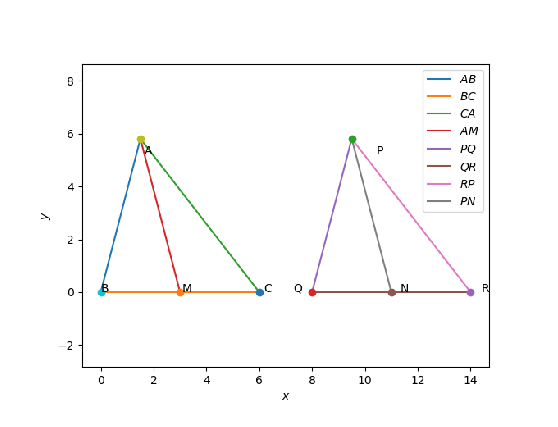
\includegraphics[width= \columnwidth]{Figure_1.eps}
\caption{Using Python}
\label{fig:circle_python}
\end{figure}
%
and the equivalent latex-tikz code for Fig. \ref{fig:circle_latex} from
\begin{lstlisting}
figs/circle.tex
\end{lstlisting}
%
The above latex code can be compiled as a standalone document as
\begin{lstlisting}
figs/circle_fig.tex
\end{lstlisting}



\end{enumerate}